% -----------------------------------------------------------------------------
% Project: PhD KAPPA
% File: kappa.Rnw (root file)
% Author: Alessio Crippa
% Template: based on the tex code written by Andrea Discacciati
%           url: https://github.com/anddis/phd-thesis
%
% Purpose: Root Rnw file, compile this to typeset the kappa!
% -----------------------------------------------------------------------------



% If you get the following error:
%  Error in ensurePackageSymlink(source, target) :
% run the next line, an then restart your R session
% unlink("packrat/lib-R", recursive = TRUE)


% Class
\documentclass[11pt,a4paper,twoside,openany]{book}\usepackage{knitr}

% Packages
\usepackage[english]{babel}
\usepackage{amsfonts}
\usepackage{amsmath}
\usepackage{mathtools}
\usepackage{threeparttable}
\usepackage{adjustbox}
\usepackage{natbib}
\usepackage{graphicx}
\usepackage{flafter}
\usepackage{fancyhdr}
\usepackage{textcomp}
\usepackage[utf8]{inputenc}
\usepackage{setspace}
\usepackage[pdftex,
            pdfauthor={Alessio Crippa},
            pdftitle={Novel methods for dose--response meta-analysis},
            pdfcreator={LaTeX2e}]{hyperref}
\usepackage[%showframe,
			headheight=13.6pt,
			%headsep=,
			%footskip=,
			bindingoffset=0cm,%print=.5cm, web=0cm
			left=3cm,  %print=2cm, web=3cm
			bottom=3cm, %print=3cm, web=3cm
			top=3cm, %print=3cm, web=3cm,
			right=3cm]{geometry} %print=3.5cm, web=3cm
\usepackage{enumerate, mdwlist}
\usepackage{etoolbox}
\usepackage{tabularx}
\usepackage{rotating}
\usepackage[font={small}]{caption}
\usepackage{chngcntr}
\counterwithout{footnote}{chapter}

%---begin see http://www.khirevich.com/latex/font/
\usepackage[activate={true,nocompatibility},final,tracking=true,kerning=true,spacing=true,factor=1100, stretch=10,shrink=10]{microtype}
% remove warning
\microtypecontext{spacing = nonfrench}
\usepackage[T1]{fontenc}
% remove warning
\global\expandafter\let\csname ver@amsfonts.sty\endcsname\relax
% remove issue related to interwordspace
\setlength{\emergencystretch}{10pt}
\usepackage[bitstream-charter]{mathdesign}
\usepackage{sectsty}
	\chapterfont{\usefont{T1}{qhv}{b}{n}\selectfont\huge}
\usepackage{titlesec}

% ---------------------------------------------------------
% Project: PhD KAPPA
% File: _titlesec.tex
% Author: Andrea Discacciati
%
% Purpose: Headings format
%			(see titlesec package)
% ---------------------------------------------------------

\titleformat{\section}[hang]{
    \usefont{OT1}{qhv}{bx}{n}\selectfont}
    {} 
    {0em}
    {\hspace{-0.4pt}\Large \thesection\hspace{0.6em}}
\titleformat{\subsection}[hang]{
    \usefont{OT1}{qhv}{bx}{n}\selectfont}
    {} 
    {0em}
    {\hspace{-4pt} \thesubsection\hspace{0.6em}}
\titleformat{\subsubsection}[hang]{
    \usefont{OT1}{qhv}{bx}{n}\selectfont}
    {} 
    {0em}
    {\normalsize}
\usepackage{tocloft}

% ---------------------------------------------------------
% Project: PhD KAPPA
% File: _tocloft.tex
% Author: Andrea Discacciati
%
% Purpose: Table of Contents, 
%			List of Figures, List of Tables format
%			(see tocloft package)
% ---------------------------------------------------------

\renewcommand{\cfttoctitlefont} % ToC title
             {\usefont{T1}{qhv}{b}{n}\selectfont\huge}
\renewcommand{\cftchapfont} % chapter titles
             {\usefont{T1}{qhv}{b}{n}\selectfont}
\renewcommand{\cftsecfont} % section titles
             {\usefont{T1}{bch}{m}{n}\selectfont}
\renewcommand{\cftsubsecfont} % subsection titles
             {\usefont{T1}{bch}{m}{n}\selectfont} 
\renewcommand{\cftchappagefont} % chapter page numbers
             {\usefont{T1}{bch}{b}{n}\selectfont}
\renewcommand{\cftsecpagefont} % section page numbers
             {\cftsecfont} 
\renewcommand{\cftsubsecpagefont} % subsection page numbers
             {\cftsubsecfont}
             
\renewcommand{\cftloftitlefont} % LoF title
             {\usefont{T1}{qhv}{b}{n}\selectfont\huge}
\renewcommand{\cftfigfont} % Figures titles
             {\usefont{T1}{bch}{m}{n}\selectfont}
             
\renewcommand{\cftlottitlefont} % LoT title
             {\usefont{T1}{qhv}{b}{n}\selectfont\huge}
\renewcommand{\cfttabfont} % Tables titles
             {\usefont{T1}{bch}{m}{n}\selectfont}
%---end see http://www.khirevich.com/latex/font/

% Header / footer

% ---------------------------------------------------------
% Project: PhD KAPPA
% File: _fancyhdr.tex
% Author: Alessio Crippa
% based on the template written by Andrea Discacciati
%
% Purpose: Header and footer settings
%			(see fancyhdr package)
% ---------------------------------------------------------

\pagestyle{fancy}
\renewcommand{\chaptermark}[1]{%
 \markboth{{\thechapter.\ #1}}{}}

\fancypagestyle{plain}{%
  \fancyhf{}%
  \renewcommand{\headrulewidth}{0pt}%
  \fancyhf[lef,rof]{}%
  %\fancyhead[LE,RO]{\thepage}
}

\fancypagestyle{frontmatter}{%
  \renewcommand{\headrulewidth}{0pt} 
  \renewcommand{\footrulewidth}{0pt}
  \fancyhf{}% Clear header/footer
  \fancyhead[LE,RO]{}
}

\fancypagestyle{nothing}{%
  \renewcommand{\headrulewidth}{0pt} 
  \renewcommand{\footrulewidth}{0pt}
  \fancyhf{}% Clear header/footer
  \fancyhead[LE,RO]{}%
}

\fancypagestyle{mainmatter}{%
  \renewcommand{\headrulewidth}{.4pt}
  \renewcommand{\footrulewidth}{0pt}
  \fancyhf{}% Clear header/footer
  \fancyhead[LE,RO]{\thepage}
  \fancyhead[RE,LO]{\nouppercase \leftmark}
}

	
% See 'writing a thesis with latex' p25 
% Writes nothing on empty pages
\makeatletter
\def\cleardoublepage{\clearpage\if@twoside
\ifodd\c@page
\else\hbox{}\thispagestyle{empty}\newpage
\if@twocolumn\hbox{}\newpage\fi\fi\fi}
\makeatother

% Substitutions (%examples)
%\newcommand{\rveplot}{decorrelated-residuals--versus--exposure plot}
%\newcommand{\kgmsq}{kg$\times$m\textsuperscript{$-2$}}

\defcitealias{crippadosresmeta2016}{Paper~I}	
\defcitealias{discacciati2015goodness}{Paper~II}	
\defcitealias{crippa2016new}{Paper~III}	
\defcitealias{crippa2018pointwise}{Paper~IV}	
\defcitealias{crippa2018one}{Paper~V}	

%\doublespacing 
\onehalfspacing

\allowdisplaybreaks

\renewcommand{\sfdefault}{qhv}
\newcommand*{\LargerCdot}{\raisebox{-0.25ex}{\scalebox{1.2}{$\cdot$}}}

\DeclareMathOperator{\R}{\textsf{R}}
\DeclareMathOperator{\Var}{Var}
\DeclareMathOperator{\Cov}{Cov} 
\DeclareMathOperator{\diag}{diag} 
\DeclareMathOperator{\N}{N} 
\DeclareMathOperator{\E}{E}
\DeclareMathOperator{\logit}{logit} 
\DeclareMathOperator{\df}{df} 
\hyphenation{logRRs}
\hyphenation{logRR}

\addto\captionsenglish{%
  \renewcommand{\bibname}{References}%
}

%\includeonly{abstract, results, introduction, background, aims, discussion, conclusions }

%--- Kappa starts here! ---%
\IfFileExists{upquote.sty}{\usepackage{upquote}}{}
\begin{document}

% Front matter
\frontmatter
\pagestyle{nothing}

% ---------------------------------------------------------
% Project: PhD KAPPA
% File: titlepage.tex
% Author: Alessio Crippa
% based on the template written by Andrea Discacciati
%
% Purpose: Custom title page + ISBN/copyright page
% ---------------------------------------------------------

\begin{titlepage}
\newgeometry{margin=4cm}
\begin{center}
\large
From the Department of Public Health Sciences \\
Karolinska Institutet, Stockholm, Sweden        
\vfill
\Large
\textbf{\textsf{NOVEL METHODS FOR DOSE-RESPONSE META-ANALYSIS}}
\vfill
\Large
Alessio Crippa
\vfill

\includegraphics[width=0.8\textwidth]{figures/ki-logo_pos}
\vfill
\large
Stockholm 2018        
\end{center}
\restoregeometry
\end{titlepage}

\newpage
\null
\vfill
\noindent All published papers reproduced with permission \\
%Cover illustration ``Portraits of sophistication'' by Lamai McCartan \\
Published by Karolinska Institutet \\
\bigskip
Printed by E-Print AB 2018 \\
Edited in R using knitr \\
\textcopyright Alessio Crippa, 2018 \\
ISBN <include number>
\newpage

% ---------------------------------------------------------
% Project: PhD KAPPA
% File: spikblad.tex
% Author: Alessio Crippa
% based on the template written by Andrea Discacciati
%
% Purpose: Spikblad
% ---------------------------------------------------------
\null
\vspace{1.5cm}
\noindent{\Large \textsf{NOVEL METHODS FOR DOSE-RESPONSE META-ANALYSIS} \vspace{1cm}}\\
\noindent{\Large \textsf{THESIS FOR DOCTORAL DEGREE (Ph.D.)} \vspace{.5cm}}\\
By \vspace{.5cm} \\
{\Large \textbf{\textsf{Alessio Crippa}} \vspace{2cm}}\\
\begin{minipage}[t]{6.2cm}
\singlespacing
{\small
\textit{Principal supervisor:}\\
Associate Professor Nicola Orsini \\
Karolinska Institutet \\
\bigskip
Department of Public Health Sciences \\
\textit{Co-supervisor:}\\
Professor Alicja Wolk \\
Karolinska Institutet \\
\medskip
Institute of Environmental Medicine \\
Professor Matteo Bottai \\
Karolinska Institutet \\
\medskip
Institute of Environmental Medicine \\
Professor Donna Spiegelman \\
Harvard T.H. Chan School of Public Health \\
Department of Epidemiology
}
\end{minipage}
\hspace{1.5cm}
\begin{minipage}[t]{8.1cm}
\singlespacing
{\small
\textit{Opponent:}\\
Professor Christopher H. Schmid \\
Brown University \\
Center for Evidence Based Medicine\bigskip \\
\textit{Examination board:}\\
Associate Professor Nele Brusselaers \\
Karolinska Institutet \\
Department of Microbiology, Tumor and Cell Biology \medskip \\
Associate Professor Antonio Gasparrini \\
London School of Hygiene and Tropical Medicine \\
Department of Social $\&$ Environmental Health Research\medskip \\
Professor Paul Lambert \\
University of Leicester \\
Department of Health Sciences
}
\end{minipage}
\cleardoublepage

% ---------------------------------------------------------
% Project: PhD KAPPA
% File: dedication.tex
% Author: Alessio Crippa
% based on the template written by Andrea Discacciati
%
% Purpose: Dedication
% ---------------------------------------------------------

\begin{flushright}
%http://pubmedcentralcanada.ca/pmcc/articles/PMC2550765/pdf/bmj00610-0065.pdf
\null\vspace{\stretch{1}}
\textit{``The function of the expert reviewer is not to be more right than other people, \\
but to be wrong for more sophisticated reasons.''} \\
---Iain Chalmers and Douglas G. Altman \\ 
\textit{Systematic Reviews}, 1995
\vspace{\stretch{2}}\null
\end{flushright}


\iffalse
\begin{flushright}
\null\vspace{\stretch{1}}
\textit{``If I have seen further, it is by standing on the shoulders of giants.''} \\
---Isaac Newton
\vspace{\stretch{2}}\null
\end{flushright}
\fi
\cleardoublepage 
\pagestyle{frontmatter}

% ---------------------------------------------------------
% Project: PhD KAPPA
% File: abstract.tex
% Author: Andrea Discacciati
%
% Purpose: Abstract frontmatter
% ---------------------------------------------------------


\noindent {\Large \textsf{\textbf{{Abstract}}}
\bigskip
%\chapter*{Abstract}
\small
\par Dose--response meta-analysis is a statistical procedure for combining and contrasting the evidence on the association between a continuous exposure and the risk of a health outcome. Several papers refined selected aspects of the methodology, such as implementation of flexible strategies and extensions to multivariate meta-analysis. However, there were still several relevant questions that needed to be addressed. This thesis aims to address these issues by developing and implementing new strategies and ad-hoc measures (\citetalias{crippadosresmeta2016}), including tools for evaluating the goodness-of-fit (\citetalias{discacciati2015goodness}), a new measure for quantifying the impact of heterogeneity (\citetalias{crippa2016new}), a strategy to deal with differences in the exposure range across studies (\citetalias{crippa2018pointwise}), and a one-stage approach to estimate complex models without excluding relevant studies (\citetalias{crippa2018one}).

In \citetalias{crippadosresmeta2016}, we described the implementation of the main aspects of the methodology in the \texttt{dosresmeta} $\R$ package available on CRAN. Dedicated functions was written to facilitate specific tasks such as definition of the design matrix and prediction of the pooled results. We illustrated how to estimate both linear and non-linear curves, conduct test of hypotheses, and present the results in a tabular and grapichal format using summarized data on alcohol intake and colorectal cancer risk.
 
In \citetalias{discacciati2015goodness}, we discussed how to evaluate the goodness-of-fit. The proposed solutions consist of descriptive measures to summarize the agreement between fitted and observed data (the deviance and the coefficient of determination), and graphical tools to visualize the fit of the model (decorrelated residuals-versus-exposure plot). A reanalysis of two published meta-analyses exemplified how these tools can improve the practice of quantitative synthesis of aggregated dose--response data. 

In \citetalias{crippa2016new}, we proposed and characterized a new measure, $R_b$, to quantify the proportion of the variance of the pooled estimate attributable to the between-study heterogeneity. Contrary to the available measures of heterogeneity, $R_b$ does not make any assumption about the distribution of the within-study error variances, nor does it require specification of a typical value for these quantities. The performance of the proposed measure was evaluated in an extensive simulation study. We demonstrated how to present and interpret the $R_b$ re-analyzing three published meta-analyses.

In \citetalias{crippa2018pointwise}, we extended a point-wise approach to dose--response meta-analysis of aggregated data. The strategy consists of combining predicted relative risks for a fine grid of exposure values based on potentially different dose--response models. A point-wise approach can improve the flexibility in modeling the study-specific curves and may limit the impact of extrapolation by predicting the study-specific relative risk based on the observe exposure range. We illustrated the methodology using both individual and aggregated participant data.

In \citetalias{crippa2018one}, we formalized a one-stage approach for dose--response meta-analysis in terms of a linear mixed model. We explained the main aspects of the methodology and how to extend the measures typically presented in a two-stage analysis. Using both hypothetical and real data, we showed how the one-stage approach can facilitate investigation the impact of heterogeneity over the exposure range, model comparison, and prediction of individual dose--response associations. The main advantage is that flexible curves can be estimated regardless of the number of data-points in the individual analyses.

In conclusion, the methods presented in this thesis enrich the set of tools available for applying dose--response meta-analyses and for addressing specific questions including goodness-of-fit evaluation (\citetalias{discacciati2015goodness}) and quantification of heterogeneity (\citetalias{crippa2016new}). In addition, we presented alternative models for pooling results in case of heterogeneous exposure range (\citetalias{crippa2018pointwise}) and for estimating complex models without excluding relevant studies (\citetalias{crippa2018one}). The proposed methods have been illustrated using real data and implemented in the \texttt{dosresmeta} and \texttt{hetmeta} $\R$ packages available on CRAN (\citetalias{crippadosresmeta2016}). 

\normalsize
\cleardoublepage

% ---------------------------------------------------------
% Project: PhD KAPPA
% File: publications.tex
% Author: Alessio Crippa
% based on the template written by Andrea Discacciati
%
% Purpose: List of publications + related publications
% ---------------------------------------------------------

\chapter*{List of publications}

\begin{enumerate}[I.]
\item Alessio~Crippa, and Nicola~Orsini \\ \textbf{Multivariate dose--response meta-analysis: the dosresmeta R Package} \\ \textit{Journal of Statistical Software, Code Snippets} 2016; 72(1), 1--15
\item Andrea~Discacciati, Alessio~Crippa, and Nicola~Orsini \\ \textbf{Goodness of fit tools for dose--response meta-analysis of binary outcomes} \\ \textit{Research Synthesis Methods} 2015
\item Alessio~Crippa, Polyna~Khudyakov, Molin~Wang, Nicola~Orsini, and Donna~Spiegelman \\ \textbf{A new measure of between-studies heterogeneity in meta-analysis} \\ \textit{Statistics in medicine} 2016; 35(21), 3661--75
\item Alessio~Crippa, Ilias~Thomas, and Nicola~Orsini \\ \textbf{A pointwise approach to dose-response meta-analysis of aggregated data} \\ \textit{Manuscript} 2018
\item Alessio~Crippa, Andrea~Discacciati, Matteo~Bottai, Alicja~Wolk, and Nicola~Orsini \\ \textbf{One-stage dose--response meta-analysis for aggregated data} \\ \textit{Manuscript} 2018
\end{enumerate}
\vspace{1.5cm}
\noindent{The articles will be referred to in the text by their Roman numerals, and are reproduced in full at the end of the thesis.}

\chapter*{Related publications}
\begin{itemize}
\item Alessio~Crippa, Susanna~C.~Larsson, Andrea~Discacciati, Alicja~Wolk, and Nicola~Orsini \\ \textbf{Red and processed meat consumption and risk of bladder cancer: a dose--response meta-analysis of epidemiological studies} \\ \textit{European journal of nutrition} 2016, 1--13
\item Andrea~D.~Smith, Alessio~Crippa, James~Woodcock, and S{\o}ren~Brage \\ \textbf{Physical activity and incident type 2 diabetes mellitus: a systematic review and dose--response meta-analysis of prospective cohort studies} \\ \textit{Diabetologia} 2016, 1--19
\item Marco~Vinceti, Tommaso~Filippini, Alessio~Crippa, Agn{\`e}s~de~Sesmaisons, Lauren~A.~ Wise, and Nicola~Orsini \\ \textbf{Meta-Analysis of Potassium Intake and the Risk of Stroke} \\ \textit{Journal of the American Heart Association} 2016, 5(10), e004210
\item Alessio~Crippa, and Nicola~Orsini \\ \textbf{Dose--response meta-analysis of differences in means} \\ \textit{BMC medical research methodology} 2016, 16(1), 91
\item Emir~Veledar, Alessio~Crippa, Chukwuemeka~U.~Osondu, Adnan~Younus, and Khurram~Nasir \\ \textbf{Letter to Editor: Ideal cardiovascular health metrics and risk of cardiovascular disease or mortality} \\ \textit{International journal of cardiology} 2016, 222, 737
\item Alessio~Crippa, Andrea~Discacciati, Nicola~Orsini, and Viktor~Oskarsson \\ \textbf{Letter: coffee consumption and gallstone disease---a cautionary note on the assignment of exposure values in dose--response meta-analyses} \\ \textit{Alimentary Pharmacology \& Therapeutics} 2016, 43(1), 166-167
\item Susanna~C.~Larsson, Alessio~Crippa, Nicola~Orsini, Alicja~Wolk, and Karl~Micha{\"e}lsson \\ \textbf{Milk consumption and mortality from all causes, cardiovascular disease, and cancer: a systematic review and meta-analysis} \\ \textit{Nutrients} 2016, 7(9), 7749-7763
\item Daniela~Di~Giuseppe, Alessio~Crippa, Nicola~Orsini, and Alicja~Wolk \\ \textbf{Fish consumption and risk of rheumatoid arthritis: a dose-response meta-analysis} \\ \textit{Arthritis research \& therapy} 2014, 16(5), 446
\item Alessio~Crippa, Andrea~Discacciati, Susanna~C.~Larsson, Alicja~Wolk, and Nicola~Orsini \\ \textbf{Coffee consumption and mortality from all causes, cardiovascular disease, and cancer: a dose--response meta-analysis} \\ \textit{American journal of epidemiology} 2014, 180(8), 763-775
\end{itemize}
\cleardoublepage
\microtypesetup{protrusion=false}
\tableofcontents
%\listoffigures
%\newpage
%\listoftables
\microtypesetup{protrusion=true} 

% ---------------------------------------------------------
% Project: PhD KAPPA
% File: abbreviations.tex
% Author: Alessio Crippa
% based on the template written by Andrea Discacciati
%
% Purpose: List of abbreviations
% ---------------------------------------------------------

\chapter*{List of abbreviations}
\begin{tabular}{ll}

AIC & Akaike Information Criterion \\
CI & Confidence Interval \\
df & Degrees of Freedom \\
GLS & Generalized Least Squares \\
GRSS & Generalized Residual Sum of Squares \\
GTSS & Generalized Total Sum of Squares \\
FP2 & Second-degree Fractional Polynomials \\
HRR & Hazard Rate Ratio \\
IR & Incidence Rate \\
IRR & Incidence Rate Ratio \\
logRR & log--Relative Risk \\
MR & Mortality Rate \\
MRR & Mortality Rate Ratio \\
RCS & Restricted Cubic Splines \\
$R^2$ & Coefficient of Determination \\
RR & Relative Risk \\
WLS & Weighted Least Squares


\end{tabular}

% Main matter
\mainmatter
\pagestyle{mainmatter}

% !TeX root = ../kappa.Rnw  


% ---------------------------------------------------------
% Project: PhD KAPPA
% File: introduction.tex
% Author: Andrea Discacciati
%
% Purpose: Introduction
% ---------------------------------------------------------

\chapter{Introduction}

A single experiment can hardly provide a definitive answer to a scientific question. Science is oftentimes referred to as a cumulative process where results from many studies, aiming to address the common question of interest, contribute to create and update the scientific evidence. In the cumulative paradigm, meta-analysis is the statistical methodology to combine and compare the current evidence in the field. This process lies at the heart of the concept of evidence-based medicine, and plays a major role in informing policy and practice.

Epidemiological studies often assess whether the occurrance of a health outcome (e.g. mortality, incidence of a disease) varies according to a quantitative exposure (e.g. amount of physical activity, alcohol intake). 
The quantitative exposure is frequently divided in intervals and the results are expressed in a tabular format as relative risks for different exposure groups. A high verusu low meta-analysis contrasts the relative risks for the highest exposure category compared to the lower one. This approach, however, discards the results for intermediate categories and thus provides only a limited picture. The information of the quantitative exposure is also lost and the estimates being compared may be associated to different exposure values.

A dose--response meta-analysis, instead, has the potential to be more informative and powerful since it uses the whole available information to estimate the dose--response association. Because the estimates depend on the same reference group, it is not possible to regress the relative risks on the assigned dose using oridinaly least square. Greenland and Longnecker described in their seminal paper in 1992 how to reconstruct the correlation within set of relative risks and incorporate it in the dose--response analysis using generalized least square regression. Since then, the number of published dose--response meta-analysis has rapidly increased in many fields of application including oncology, public health, environmental sciences, nutrition, endocrinology, and internal medicine. 
Additional papers refined selected aspects of the proposed methodology, mainly focusing on the implementation of flexible strategies in modeling non-linear associations and incorporating the advances of multivariate meta-analysis. However, there were still several relevant questions that needed to be addressed such as how to assess the goodness-of-fit (\citetalias{discacciati2015goodness}), how to quantify the impact of heterogeneity (\citetalias{crippa2016new}, how to deal with differences in the exposure range across studies (\citetalias{crippa2018pointwise}), and how to estimate complex models without excluding relevant studies (\citetalias{crippa2018one}).

%This thesis aims to address these issues by developing and implementing new strategies and ad-hoc measures (\citetalias{crippadosresmeta2016}), including tools to evaluate the goodness-of-fit (\citetalias{discacciati2015goodness}), a new measure to quantify the impact of heterogeneity (\citetalias{crippa2016new}), a strategy to deal with differences in the exposure range across studies (\citetalias{crippa2018pointwise}), and a one-stage approach to estimate complex models without excluding relevant studies (\citetalias{crippa2018one}).
This thesis aims to address these issues by developing and implementing new strategies and ad-hoc measures (\citetalias{crippadosresmeta2016}). The proposed methodologies are demonstrated reanalyzing published meta-analyses and are implemented in user friendly packages written in the free and open source R language, to bridge the gap between theory and application.

% !TeX root = ../kappa.Rnw  

% ---------------------------------------------------------
% Project: PhD KAPPA
% File: background.tex
% Author: Alessio Crippa
% based on the template written by Andrea Discacciati
%
% Purpose: Background
% ---------------------------------------------------------

\chapter{Background}

\section{Meta-analysis}

Relevant research questions are typically addressed by independent investigators in multiple studies. The sampling error and possibly differences in the investigations will inevitably produce diverse results, sometimes even conflicting. Evidence-based medicine requires a synthesis of the available evidence to optimize the decision-making process \citep{haidich2010meta}. 

Meta-analysis, or more generally quantitative review synthesis, is the statistical methodology for integrating and synthetizing the information arising from multiple studies \citep{borenstein2009references}. Using appropriate statistical models, quantitative reviews contrast and pool results in the hope of identifying similarities or explain differences across study findings. Meta-analysis represents the state of the art for systematically reviewing the evidence, as indicated by the increasing number of published meta-analyses over the last 40 years (Figure~\ref{fig:num_meta-analysis}).

The classical approach for meta-analysis consists of a weighted average of the study-specific results or estimates. A fixed-effect model for meta-analysis assumes that all the studies estimate a single common parameter \citep{rice2017re}. The hypothesis of homogeneity of the estimates is rarely applicable in biomedical and social sciences where studies typically differ in terms of design, disease classification, exposure measurement, and implemented statistical analyses \citep{colditz1995heterogeneity}. In such cases, heterogeneity across estimates is expected and should be considered in the analysis \citep{higgins2009re}. If the parameters estimated in the studies are not identical but similar, a random-effects models can be used to identify those similarities or to explain the observed heterogeneity \citep{higgins2009re}.


\begin{knitrout}
\definecolor{shadecolor}{rgb}{0.969, 0.969, 0.969}\color{fgcolor}\begin{figure}[ht!]

{\centering \includegraphics[width=\textwidth]{../figure/num_meta-analysis-1} 

}

\caption[Number of publications about meta-analysis (results from Medline search using text "meta-analysis" until December 2017)]{Number of publications about meta-analysis (results from Medline search using text "meta-analysis" until December 2017).}\label{fig:num_meta-analysis}
\end{figure}


\end{knitrout}


\subsection{Random-effects meta-analysis}

In a meta-analysis of $K$ studies indexed by $i = 1, \dots, K$, we denote $\hat \beta_i$ the estimate of an effect of interest (effect size) in the $i$-th study.
%, and $\hat v_i$ an estimate of the related sampling variance. 

A random-effects model for meta-analysis can be written as
\begin{equation}
\hat \beta_i = \beta + u_i + \varepsilon_i
\label{eq:rma}
\end{equation}

\noindent where $\beta$ is the underlying mean effect, oftentimes the main parameter of interest. The random-effects $u_i$ represent the study-specific deviations from the mean effect $\beta$ allowing each study to estimate a similar parameter $\beta_i$ defined as $\beta + u_i $. The random component follows a generic $f$ distribution with mean 0 and variance equal to $\tau^2$, the between-studies heterogeneity. 
The within-study error components $\varepsilon_i$ have also mean 0 and variance equal to $\hat v_i$, an estimate of the sampling variance of $\hat \beta_i$.
Because the sample size in the individual investigations is often large, the uncertainty around the estimates of the sampling variance is negligible. Therefore, $\hat v_i$ can be considered fixed and denoted as $v_i$. In addition, for the central limit theorem, $\varepsilon_i \sim  \mathcal{N}\left(0, v_i \right)$, or alternatively, $\hat \beta_i | u_i \sim \mathcal{N}\left(\beta+u_i, v_i \right)$.

An inverse variance-weighted approach for meta-analysis estimates the mean effect $\beta$ as a weighted average of the $\hat \beta_i$ \citep{whitehead1991general, dersimonian1986meta}
\begin{align}
\hat \beta = \frac{\sum_{i = 1}^k \hat \beta_i \hat w_i}{\sum_{i = 1}^k \hat w_i} \label{eq:avgbeta} \\
\widehat{\Var} \left(\hat \beta \right) = \left( \sum_{i = 1}^k \hat w_i \right)^{-1}
\end{align}
\noindent with weights $\hat w_i = \left(v_i + \hat \tau^2 \right)^{-1}$ and $\hat \tau^2$ being an estimate of the between-study heterogeneity. 


\subsection{Test and estimates of heterogeneity}

A second parameter of interest, often overlooked, is the between-study heterogeneity, $\tau^2$. Focusing on the mean effect alone may provide only a limited piece of information, especially in case of heterogeneous effects \citep{borenstein2010basic}. Indeed, an evaluation of the extent of heterogeneity is a crucial step in determining the appropriateness of presenting a summary measure of the observed effect sizes.

Presence of heterogeneity is frequently defined as the excess in the variability of $\hat \beta_i$ above that expected alone by chance. A summary measure of the observed variability is represented by the $Q$~statistic
\begin{equation}
Q = \sum_{i=1}^K \left(\hat \beta_i - \hat \beta_{\text{fe}} \right)^2
\label{eq:Q}
\end{equation}
\noindent where $\hat \beta_{\text{fe}} = \sum_{i=1}^K \hat \beta_i v_i^{-2}/ \sum_{i=1}^K v_i^{-2}$ is the estimate of $\beta$ in a fixed-effect model. Based on that, Cochrane developed a test for assessing hypothesis of homogeneity of the study-specific estimates \citep{cochran1954combination}. Under the null hypothesis of no heterogeneity ($H_0: \tau^2 = 0$) the $Q$~statistic follows a $\chi^2$ with $K-1$ degrees of freedom. A $p$~value less than 0.10 is oftentimes used as evidence for presence of between-studies variability. It is known, however, that the test is sensible to the number of studies $K$ failing to reject the null hypothesis even for high value of $\tau^2$ when K is small, and contrary it is more likely to reject $H_0$ for negligible between-studies variation when $K$ is big \citep{higgins2002quantifying, takkouche1999evaluation}. Therefore, failing to reject the null hypothesis does not provide evidence supporting homogeneity in the effect sizes \citep{biggerstaff1997incorporating}. In addition, the dichotomization heterogeneous/homogeneous is not very informative, especially because heterogeneity is almost always present. 

An estimate of $\tau^2$, instead, directly provides information about the amount of heterogeneity and is thus the more natural measure of between-studies variability. Based on the expectation of $Q$, Dersimonian and Laird proposed the following estimator for $\tau^2$ using the method of moments \citep{dersimonian1986meta}
\begin{equation}
\hat \tau^2_{\text{DL}} = \max \left\{0, \frac{Q - (K-1)}{\sum_{i=1}^K v_i^{-2} - \sum_{i=1}^K v_i^{-4}/\sum_{i=1}^K v_i^{-2} } \right\}
\label{eq:tau2DL}
\end{equation}

\noindent The moment-based estimator is one of the most popular estimators of $\tau^2$ because it has a simple non-iterative formulation and does not require any distributional assumptions for the random-effects rather than having a finite first order moment. Other common non-iterative alternatives include an estimator based on the variance components \citep{hedges1983random} and using methods for estimating the error variance in a weighted linear model \citep{sidik2005simple}. Iterative methods based on maximizing the likelihood or restricted likelihood can also be used by specifying a distributional form for the random-effects. The more conventional choice is typically a normal distribution $u_i \sim \mathcal{N}\left( 0, \tau^2 \right)$, which implies $\beta_i \sim \mathcal{N}\left(\beta, \tau^2 \right)$ and $\hat \beta_i \sim \mathcal{N}\left(\beta + u_i, \tau^2 + v_i \right)$.

Although $\tau^2$ is the more natural and appropriate measure of between-study variability, the actual value is difficult to interpret because it depends on type of effect size (e.g. log relative risk, standardized mean difference) and has no upper limit. Therefore, both evaluation of the degree (or levels) and the comparison of heterogeneity in different meta-analyses can hardly be based on the estimate of $\tau^2$.


\subsection{Measures of heterogeneity}

To complement the test based approach and the information provided by $\hat tau^2$, measures that quantify the impact of heterogeneity have been proposed \citep{higgins2002quantifying}. 
Higgins et al. presented several possibilities in the simpler case where all the sampling variances $v_i$ are equal to a fixed and known value $\sigma^2$. 

Two measures aim to estimate the ratio $\sigma^2/(\sigma^2/ + \tau^2)$, namely the $H^2= Q/(K-1)$ that represents the excess in $Q$~statistic relative to its degrees of freedom, and $R^2 = \Var{\hat \beta}/\Var{\hat \beta_{\text{FE}}}$ which describe the inflation in the variability of the mean effect in a random-effects model compared with a fixed-effect model.
Other measures, instead, relate the between-studies heterogeneity, $\tau^2$, to the marginal or unconditional variability $\tau^2 + v_i$, which is defined by the sum of within- and between-study components. These measures can be more easily interpreted as the percentage of the total variability due to heterogeneity, similar to the intraclass correlation coefficient defined for linear mixed-effects models. The ratio directly involves the within-terms $v_i$ that again varies across the studies. Indeed, the most popular measures, namely the $R_I$ \citep{ takkouche1999evaluation} and the $I^2$ \citep{higgins2002quantifying}, replaced $v_i$ with a statistic that summarizes the observed distribution of $v_i$.
Takkouche et al. chose
\begin{equation}
s_1^2 = \frac{K}{\sum_{i=1}^K v_i^{-2}}
\label{eq:Ri}
\end{equation}
\noindent that is the harmonic mean of the inverse of the sampling variances. 
Higgins et al., instead, described the ``typical'' within-study variance as
\begin{equation}
s_2^2 = \frac{(K-1) \sum_{i=1}^K v_i^{-2}}{ \left( \sum_{i=1}^K v_i^{-2} \right)^2 - \sum_{i=1}^K v_i^{-4}}
\label{eq:I2}
\end{equation}
\noindent that provided a direct relationship with the $Q$~statistic: $I^2 = (Q - (K-1))/Q$ when $\tau^2$ is estimated using the method of moments.
\noindent Both statistics can be expressed as a percentage where 0\% corresponds to no heterogeneity and increasing values imply higher levels of heterogeneity. It is known that these measures depend on precision of the study-specific estimates and tend to increase to 100\% when the $v_i$ are much smaller than the estimated $\tau^2$. 
A complementary measure is the between-studies coefficient of variation, defined as $\tau^2/|\hat \beta|$, that does not directly depend on the within-study variances. However, it increases quickly as $\hat \beta$ becomes smaller, and is not defined for $\hat \beta = 0$.

While the limitations of the $Q$~test approach are widely known, little emphasis is placed on the assumptions underneath the definition of the established measures of heterogeneity, i.e.  all the estimates being reported with the same precision, which is unlikely to be met in almost all the applications. A measure of the impact of heterogeneity that does not require such an assumption would be desirable.


\section{Categorical models for dose--response analysis}





\newpage

\subsection{Categorical analysis with individual participant data}

\subsection{Aggregated dose--response data}

\subsection{High versus low meta-analysis}



\section{Dose--response meta-analysis}

\subsection{First stage: study-specific curves}

\subsection{Second stage: multivariate meta-analysis}



\section{Software}



Here an example of a figure (Figure~\ref{fig:cite_grl}).

\begin{knitrout}
\definecolor{shadecolor}{rgb}{0.969, 0.969, 0.969}\color{fgcolor}\begin{figure}[ht!]

{\centering 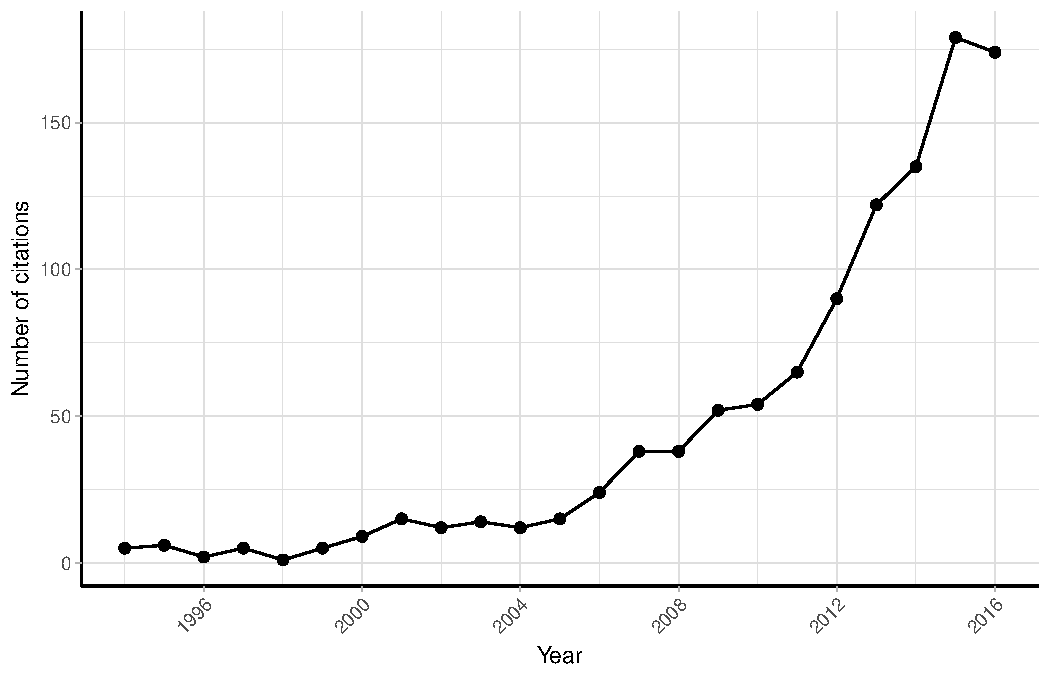
\includegraphics[width=\textwidth]{../figure/cite_grl-1} 

}

\caption[Number of citations of the paper by Greenland and Longnecker (1992) obtained from Google Scholar 1992-2017 (until December 2017)]{Number of citations of the paper by Greenland and Longnecker (1992) obtained from Google Scholar 1992-2017 (until December 2017).}\label{fig:cite_grl}
\end{figure}


\end{knitrout}


% !TeX root = ../kappa.Rnw  


% ---------------------------------------------------------
% Project: PhD KAPPA
% File: aims.tex
% Author: Alessio Crippa
% based on the template written by Andrea Discacciati
%
% Purpose: Aims
% ---------------------------------------------------------

\chapter{Aims of the thesis}

The overall aims of this thesis were to develop and implement new methods for dose--response in meta-analysis, in order to deal with the methodological aspects that have not yet been addressed.

\bigskip

More specifically, the aims were:

\begin{itemize}
\item To describe the implementation of the main aspects of a dose--response meta-analysis and the usage of the \texttt{dosresmeta} $\R$ package.

\item To present and discuss relevant measures and graphical tools to assess the goodness-of-fit in dose--response meta-analysis.

\item To develop a new measure of between-study heterogeneity in the broader context of meta-analysis and assess its properties as compared to other available measures. 

\item To explore possible advantages of a point-wise approach, especially, in case of dose--response meta-analysis where the exposure range varies substantially across the studies.

\item To formalize and present an alternative one-stage random-effects model for dose--response meta-analysis of aggregated data, formulating the meta-analytic model in terms of a general linear mixed-effect model. 

\end{itemize}

% !TeX root = ../kappa.Rnw  


% ---------------------------------------------------------
% Project: PhD KAPPA
% File: materials.tex
% Author: Alessio Crippa
% based on the template written by Andrea Discacciati
%
% Purpose: Materials
% ---------------------------------------------------------

\chapter{Methods}

\section{The \texttt{dosresmeta} R package}

\subsection{Implementation}

\subsection{Exposure modeling}


\section{A new measure of heterogeneity}

\subsection{Statistical proporties}

\subsection{Simulation study}


\section{Goodness-of-fit}

\subsection{Deviance}

\subsection{Coefficient of determination}

\subsection{Visual tools}


\section{A point-wise approach}

\subsection{Prediction of study-specific (log) relative risks}

\subsection{Pool of dose--response prediction}


\section{A one-stage model}

\subsection{Model definition}

\subsection{Estimation and hypothesis testing}

\subsection{Prediction}

\subsection{Comparison with two-stage analysis}

% !TeX root = ../kappa.Rnw  

% ---------------------------------------------------------
% Project: PhD KAPPA
% File: results.tex
% Author: Alessio Crippa
% based on the template written by Andrea Discacciati
%
% Purpose: Results
% ---------------------------------------------------------

\chapter{Results}




% Paper I
%\input{results.1}

% !TeX root = ../kappa.Rnw  

% ---------------------------------------------------------
% Project: PhD KAPPA
% File: discussion.tex
% Author: Alessio Crippa
% based on the template written by Andrea Discacciati
%
% Purpose: Discussion
% ---------------------------------------------------------

\chapter{Discussion}

Write the discussion with subsections as in the background section

% !TeX root = ../kappa.Rnw  

% ---------------------------------------------------------
% Project: PhD KAPPA
% File: conclusions.tex
% Author: Alessio Crippa
% based on the template written by Andrea Discacciati
%
% Purpose: Conclusions
% ---------------------------------------------------------

\chapter{Conclusions}

The methods presented in this thesis enrich the set of tools available for applying dose--response meta-analyses and for addressing specific questions including how to evaluate the goodness-of-fit and how to measure the impact of the between-studies heterogeneity. Furthermore, this thesis describes alternative models for pooling results in case of heterogeneous exposure range and for estimating complex models without excluding relevant studies. The proposed methods have been illustrated using real data from published meta-analyses and implemented in the \texttt{dosresmeta} and \texttt{hetmeta} $\R$ packages available on CRAN. 

More specifically we conclude the following:

\begin{itemize}

\item The \texttt{dosresmeta} $\R$ package can help practitioners to conduct dose--response meta-analyses and to apply the methods presented in this thesis. Dedicated functions help to avoid pitfalls frequently encountered in published meta-analyses, such as definition of the design matrix and prediction of the pooled results (\citetalias{crippadosresmeta2016}).

\item Goodness-of-fit should be regularly evaluated in applied dose--response meta-analysis. The proposed solutions consist of descriptive measures to summarize the agreement between fitted and observed data (the deviance and the coefficient of determination), and graphical tools to visualize the fit of the model (decorrelated residuals-versus-exposure plot). These tools can be employed to identify systematic dose--response patterns and possible source of heterogeneity, and to support the conclusions in applied meta-analyses (\citetalias{discacciati2015goodness}).

\item The new measure of heterogeneity, $R_b$, quantifies the proportion of the variance of the pooled estimate attributable to the between-study heterogeneity. Contrary to the available measures of heterogeneity, it does not make any assumption about the distribution of the within-study error variances, nor does it require specification of a typical value for these quantities. Therefore, we recommend the use of the $R_b$ as preferred measure for quantifying the impact of heterogeneity (\citetalias{crippa2016new}). 

\item A point-wise strategy for dose--response meta-analysis does not require the specification of a unique model as in the traditional approaches, and therefore allows for more flexibility in modeling the individual curves. In addition, the extent of extrapolation is limited by predicting the study-specific relative risk based on the observe exposure range. The use of the described strategy may improve the robustness of the results, especially in case of heterogeneous exposure range (\citetalias{crippa2018pointwise}).

\item A one-stage approach for dose--response meta-analysis consists of a linear mixed-effects model, which offer useful tools for describing the impact of heterogeneity over the exposure range, for comparing the fit of different models, and for predicting individual dose--response associations. Thhe main advantage is that flexible curves can be estimated regardless of the number of data-points in the individual analyses (\citetalias{crippa2018one}).

\end{itemize}

% !TeX root = ../kappa.Rnw  

% ---------------------------------------------------------
% Project: PhD KAPPA
% File: future.tex
% Author: Alessio Crippa
% based on the template written by Andrea Discacciati
%
% Purpose: Future research
% ---------------------------------------------------------

\chapter{Future research}

Based on the conclusions presented in this thesis, future research includes: 

\begin{itemize}
\item <>

\item <>

\item <>
\end{itemize}

% Appendix
\appendix

% !TeX root = ../kappa.Rnw  

% ---------------------------------------------------------
% Project: PhD KAPPA
% File: appendix.tex
% Author: Alessio Crippa
% based on the template written by Andrea Discacciati
%
% Purpose: Appendix
% ---------------------------------------------------------

\chapter{Supplementary figures}

Figures.

%--tables
\chapter{Supplementary tables}

Tables.

% Back matter
\backmatter
\bibliographystyle{style/jss}
\refstepcounter{chapter}
\addcontentsline{toc}{chapter}{\bibname}
\bibliography{additional/kappa_bib}
\newpage
\pagestyle{nothing}

% ---------------------------------------------------------
% Project: PhD KAPPA
% File: acknowledgements.tex 
% Author: Alessio Crippa
% based on the template written by Andrea Discacciati
%
% Purpose: Acknowledgements
% ---------------------------------------------------------

\chapter{Acknowledgements}

There are many people that I would like to thank for their contributions to this thesis, and for their support and encouragement during these years.

\bigskip

\textbf{Nicola Orsini}, my main supervisor for the second half of my doctoral education.

\bigskip

\noindent This work was supported by \textbf{Karolinska Institutet}'s funding for doctoral students (KID-funding).







\end{document}
